\section{}
Consider the electronic circuit illustrated below:

\begin{figure}[h]
    \centering
    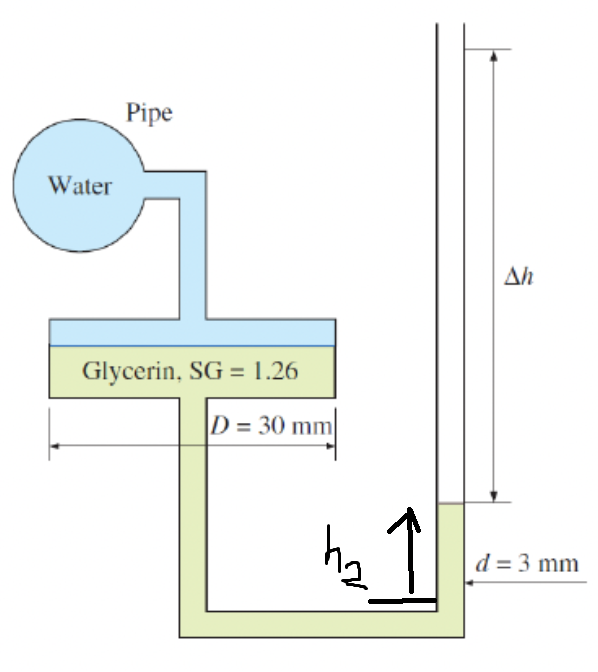
\includegraphics[width=0.5\textwidth]{Questions/Figures/Q3ProblemDiagram.png}
    \caption{Electronic RLC circuit.}
    \label{fig:Q3 System}
\end{figure}
\FloatBarrier
The states of the system are chosen as the voltage drop across the capacitor $x_1$ and the current flow 
through the inductor $x_2$. The input of the system is the voltage $u$ and the output is the voltage drop 
$y$ across resistor $R_2$. Derive the (linear) state-space form of this system.\\

In addition, let 
\begin{itemize}
    \item $V_{R}$ be the voltage drop across resistor $R$
    \item $V_{C}$ be the voltage drop across capacitor $C$
    \item $V_{L}$ be the voltage drop across inductor $L$
\end{itemize}

The governing equations for the for components of the circuit are:
\begin{align}
    V_{R} &= R i_R \\
    i_{C} &= C \frac{dV_{C}}{dt} \\
    V_{L} &= L \frac{di_{L}}{dt}
\end{align}

Performing KVL on the circuit, we get two equations:
\begin{align}
    u &= x_1 + V_{R1} \label{eq:KVL1} \\
    u &= V_{L} + V_{R2} \label{eq:KVL2}
\end{align}

By KCL, $i_{R1} = i_{C}$. Further manipulation of (\ref{eq:KVL1}) yields:
\begin{align}
    u   &= x_1 + R_{1}i_{C} \\
        &= x_1 + R_{1}C \frac{dV_{C}}{dt} \\
        &= x_1 + R_{1}C \dot{x_1}
\end{align}

By KCL, $x_2 = i_{L} = i_{R2}$. Further manipulation of (\ref{eq:KVL2}) yields:
\begin{align}
    u   &= V_{L} + R_{2}i_{L} \\
        &= L \frac{di_{L}}{dt} + R_{2}i_{L} \\
        &= L \dot{x_2} + R_{2}x_2 
\end{align}

The state space form is therefore:
\begin{empheq}[box=\fbox]{align*}
    x &=
    \begin{bmatrix}
        \dot{x_1} \\
        \dot{x_2}
    \end{bmatrix}
    =
    \begin{bmatrix}
        -\frac{1}{CR_{1}} & 0 \\
        0 & -\frac{R_{2}}{L}
    \end{bmatrix}
    \begin{bmatrix}
        x_1 \\
        x_2
    \end{bmatrix}
    +
    \begin{bmatrix}
        \frac{1}{C R_{1}} \\
        \frac{1}{L} 
    \end{bmatrix}
    \begin{bmatrix}
        u
    \end{bmatrix} \\
    y &= 
    \begin{bmatrix}
        0 & R_2
    \end{bmatrix}
    \begin{bmatrix}
        x_1 \\
        x_2
    \end{bmatrix}
\end{empheq}
